\section{Auswertung}

\subsection{Charakteristik des Geiger-Müllerzählrohrs}

Die gemessenen Daten zur Charakteristik des Geiger-Müllerzählrohrs sind in der Tabelle \ref{tab:ogemessdaten}
angegeben. Dabei ist die Zählrate poissonverteilt und lässt sich gemäß  \ref{eqn:fehlerzählrate} berechnen.
\newline
Zunächst sollen die Messpunkte mit einem Fehlerbalken in ein Diagramm eingezeichnet werden und anschließend soll entlang des Plateau-Bereiches
eine lineare Ausgleichsgerade erstellt werden. Graphisch lässt sich der Plateau-Bereich, also der Bereich in der die Zählrate kaum zunimmt bei ansteigender angelegten Spannung, grob
als Intervall von $\SI{400}{\volt}$ bis $\SI{630}{\volt}$ festlegen. Durch dieses Intervall kan nun eine lineare Ausgleichsgerade mit folgendem Ansatz gewählt werden.

\begin{equation}
y = a \cdot x + b
\end{equation}
wobei $a$ die Steigung der Geraden und $b$ der $y$-Achsenabschnitt ist.
Durch einen linearen Fit lassen sich die Parameter bestimmen zu

\begin{align}
a &= \SI{1.138(241)}{{\text{Imp}}\per(\volt\cdot{60}\second)} \\
b &= \SI{9590.735(121824)}{{\text{Imp}}\per{60}\second}
\end{align}

\begin{flushleft}
Die Messwerte mit Fehlerbalken sowie die ermittelte Ausgleichsgerade sind in dem Diagramm
\ref{fig:plot1} dargestellt.

Die Plateau-Steigerung in $\si{\percent\per{100}\volt}$ kann nun nach Wahl zweier Werte im Abstand von $\SI{100}{\volt}$ innerhalb
des Plateau-Bereiches bestimmt werden. Im folgenden wird dies durch die Zählraten zu den Spannungsumstellungen $U = \SI{400}{\volt}$ und
$U = \SI{500}{\volt}$ getan.

Für die Prozentuale Steigung $a_{\si{\percent}}$ gilt 

\begin{equation}
a_{\si{\percent}} = 100 \cdot\left( \frac{N_{500} - N_{400} }{N_{500}} \right) \si{\percent}
\end{equation}

Da die Messwerte allerdings fehlerbehaftet sind gilt die Gaußsche Fehlerfortpflanzung. Dadurch lässt sich
ein $\increment a_{\si{\percent}}$ folgendermaßen bestimmen.

\begin{align}
\increment a_{\si{\percent}} &= \sqrt{\left(\frac{\symup{d}a_{\si{\percent}}}{\symup{d}N_{500}}\right)^{2} \cdot 
(\increment N_{500})^{2} + \left(\frac{\symup{d}a_{\si{\percent}}}{\symup{d}N_{400}}\right)^{2} \cdot
(\increment N_{400})^{2}} \\
\increment a_{\si{\percent}} &= \frac{100}{N_{500}}\sqrt{\left(\frac{N_{400}}{N_{500}}\right)^{2} \cdot 
(\increment N_{500})^{2} +
(\increment N_{400})^{2}}
\end{align}

Nach dem Einsetzen der folgenden Werte

\begin{table}
\centering
\caption{Zählraten und Fehler.}
\label{tab:ogemessdaten2}
\begin{tabular}{c c c}
    \toprule
    Spannung $U$[$\si{\volt}$] & Zählrate $N$[$\text{Imp}\si{\per{60}\second}$] & Fehler $\increment N$[$\text{Imp}\si{\per{60}\second}$]\\
    \midrule
    400   & 9995 & 99{,}97\\
    500	  & 10151 & 100{,}75\\
    \bottomrule
\end{tabular}
\end{table}

Findet sich die prozentuale Steigerung $a_{\si{\percent}}$

\begin{equation}
a_{\si{\percent}} = \SI{1.5(14)}{\percent}
\end{equation}

\end{flushleft}
\begin{figure}[h]
  \centering
  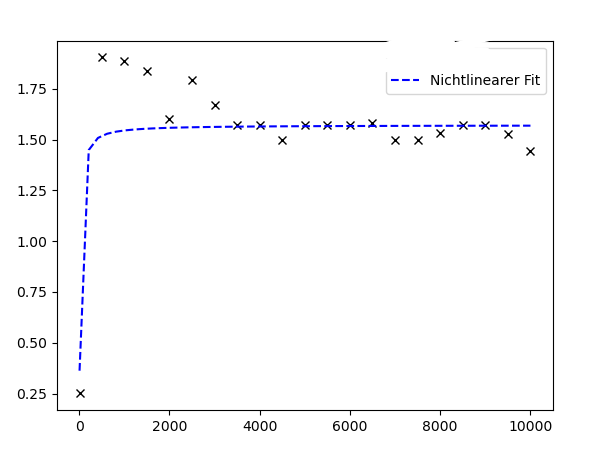
\includegraphics[width=\textwidth]{build/plot1.pdf}
  \caption{Messdaten und Fehlerbalken der Geiger-Müller Charakteristik}
  \label{fig:plot1}
\end{figure}